\documentclass[../../main.tex]{subfiles}

%-----------------------------------------------------------%
\begin{document}
\chapter{Testing \& Results}
\thispagestyle{fancy}


%-----------------------------------------------------------%
\section{Mechanical}
\blindtext
%----------------------------END----------------------------%

%-----------------------------------------------------------%
\section{Instrumentation}
For testing and learning purpose Instrumentation subsystem will first procure inexpensive components and will perform experiments to gain hands-on experience.
\subsection{Image sensor}
    OV7670
    \\The OV7670 is a low voltage CMOS image sensor which provide full functionality of single chip VGA camera.
\subsection{Lens}
    Lens system used in quadcopters, RC planes having similar lens configuration will be used to test our obtained numbers
\subsection{Baffle}
    In order to test if a baffle has been correctly manufactured or not, it has to be tested for its sun exclusion angle. The methodology developed for testing the baffle is as follows:
\begin{itemize}
    \item Acquire a Lay Susan (a simple rotating table that has been modified according to the demands of the testing procedure) and a simple light source (a light bulb should suffice)
    \item The baffle should be placed on the Lazy Susan in a dark room
    \item A sensor should be placed at the baffle entrance
    \item Place the light source in line with sensor center at 0$^\circ$
    \item Start rotating the baffle slowly till the sensor detects no light. This angle should be approximately equal to the sun exclusion angle
\end{itemize}
\par
The Lazy Susan to be used has been designed in SolidWorks and includes customization that aids in the testing process.

\begin{figure}[h]
    \centering
    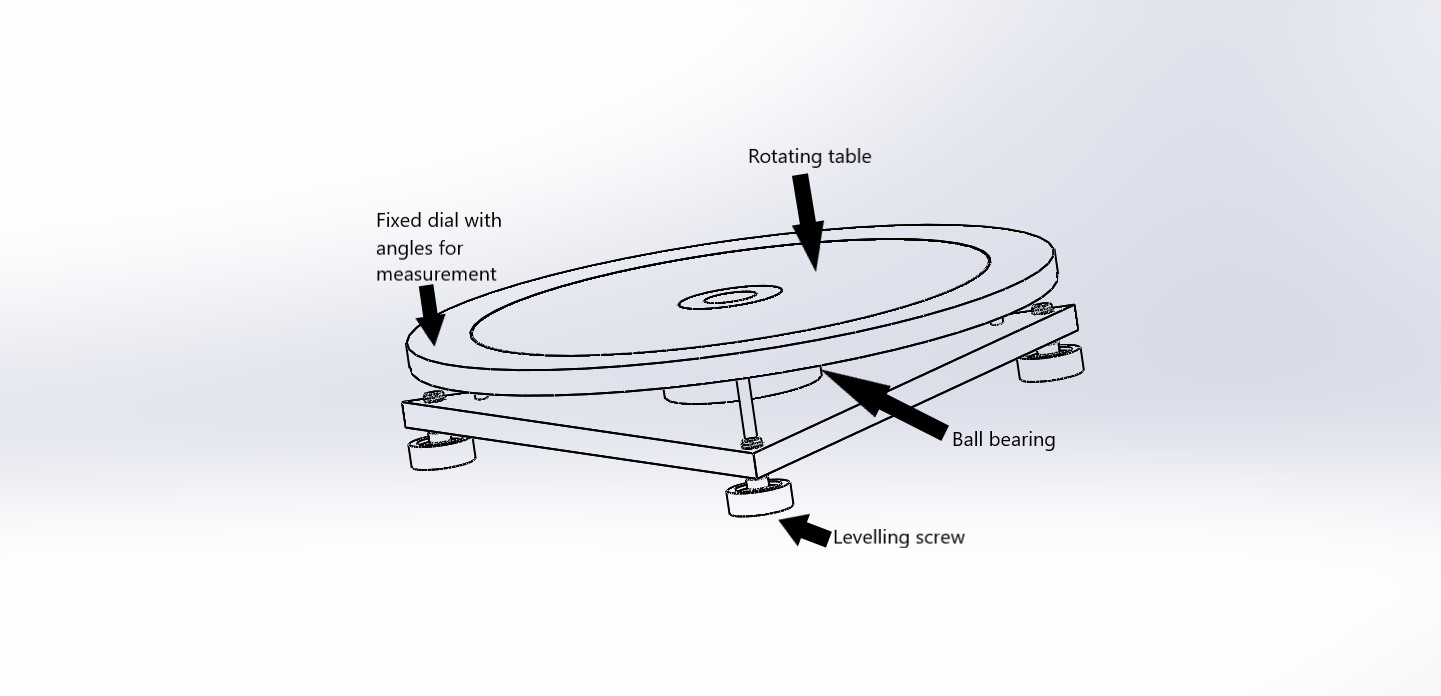
\includegraphics[width=\textwidth]{Figures/Instrumentation/lazy_susan.jpg}
    \caption{Lazy Susan apparatus for testing the baffle's sun exclusion angle}
    \label{fig:13.1}    
\end{figure}

%----------------------------END----------------------------%


%-----------------------------------------------------------%
\section{Electrical} \label{sec:Electrical_test}
\subfile{Chapters/Testing/FeatureExtraction}
%----------------------------END----------------------------%
\end{document}